%----------------------------------------------------------------------------------------
%    PACKAGES AND THEMES
%----------------------------------------------------------------------------------------

\documentclass[aspectratio=169,xcolor=dvipsnames]{beamer}
\usetheme{SimpleDarkBlue}

\usepackage{hyperref}
\usepackage{graphicx} % Allows including images
\usepackage{booktabs} % Allows the use of \toprule, \midrule and \bottomrule in tables
\usepackage{tikz}
\usetikzlibrary{decorations.pathreplacing}
\usetikzlibrary{shapes, arrows, positioning}

% --- HYPERLINKS & COLORS ---
\usepackage{hyperref}
\definecolor{NavyRed}{RGB}{140, 28, 35}
\hypersetup{
    colorlinks=true,
    linkcolor=NavyRed,  % Color for internal links (roadmap, sections)
    urlcolor=NavyRed,   % Color for external URLs
    citecolor=blue,
    filecolor=NavyRed
}

% set colors
\definecolor{hkustyellow}{RGB}{167, 131, 55}
\definecolor{hkustblue}{RGB}{120, 37, 35}
\definecolor{hkustred}{RGB}{209, 51, 59}

% --- CITATION STYLE ---
\usepackage[round]{natbib}


%----------------------------------------------------------------------------------------
%    CUSTOM NAVIGATION HEADLINE
%----------------------------------------------------------------------------------------

% 1. Set the Banner Colors
\setbeamercolor{section in head/foot}{bg=NavyRed, fg=white}

% 2. Style the Dots (Mini Frames)
\setbeamercolor{mini frame}{fg=white}
\setbeamercolor{section in head/foot shaded}{fg=white!50!NavyRed}

% 3. Define the Headline Template
\setbeamertemplate{headline}{%
  \leavevmode%
  \begin{beamercolorbox}[wd=\paperwidth,ht=2.3ex,dp=2.5ex]{section in head/foot}%
    % --- Force links to be white only inside this banner ---
    \hypersetup{linkcolor=white}% 
    \insertnavigation{\paperwidth}%
  \end{beamercolorbox}%
}

% 4. Custom Footer with Author, Title, Date, and Page Numbers
\definecolor{MiddleRed}{RGB}{160, 50, 45} % Lighter red for footer strip
\setbeamercolor{footlinebox}{bg=lightgray, fg=black}
\setbeamercolor{footlinemiddle}{bg=MiddleRed, fg=white}

\setbeamertemplate{footline}{%
  \leavevmode%
  \hbox{%
  % Left section: Author
  \begin{beamercolorbox}[wd=.25\paperwidth,ht=2.5ex,dp=1.125ex,center]{footlinebox}%
    \insertshortauthor
  \end{beamercolorbox}%
  % Middle section: Title
  \begin{beamercolorbox}[wd=.5\paperwidth,ht=2.5ex,dp=1.125ex,center]{footlinemiddle}%
    \hypersetup{linkcolor=white}%
    \insertshorttitle
  \end{beamercolorbox}%
  % Right section: Date and Frame Number
  \begin{beamercolorbox}[wd=.25\paperwidth,ht=2.5ex,dp=1.125ex,right]{footlinebox}%
    \insertshortdate{}\hspace*{2em}
    \insertframenumber{} / \inserttotalframenumber\hspace*{2ex}
  \end{beamercolorbox}}%
  \vskip0pt%
}

%----------------------------------------------------------------------------------------
%    TITLE PAGE
%----------------------------------------------------------------------------------------

\title[Context-Based Interpretation of Fin. Info.]{Context-Based Interpretation of Financial Information}
\subtitle{Kim, A. G., \& Nikolaev, V. V. (JAR 2024)}

\author[Jayden Liu]{Presenter: Jayden Liu}

\institute
{
    School of Accounting and Finance, HK PolyU % Your institution for the title page
}
\date{\today} % Date, can be changed to a custom date

%----------------------------------------------------------------------------------------
%    PRESENTATION SLIDES
%----------------------------------------------------------------------------------------

\begin{document}

% SLIDE 1: Title
\begin{frame}
    \titlepage
\end{frame}

% SLIDE 2: Roadmap
\begin{frame}{Roadmap}
    \tableofcontents
\end{frame}


% Introduction --- --- --- --- --- --- --- --- --- --- --- --- 
\section{Introduction}

\begin{frame}{Motivation}
    \begin{itemize}
        \item \textbf{Multimodal Disclosures:} Firms communicate performance using both financial numbers and narrative text.
        \item \textbf{Regulatory Requirement:} The SEC requires \textbf{MD\&A} to provide nonquantitative context to help investors accurately interpret financial results.
        \item \textbf{Standard-Setter Objective:} The SEC and IASB are actively seeking ways to improve how narrative disclosures complement numeric data.
    \end{itemize}
\end{frame}

\begin{frame}{Motivation: Financial Numbers and Narrative Text}
An example of AAPL's financial numbers and narrative text: 
    \begin{figure}
        \centering
        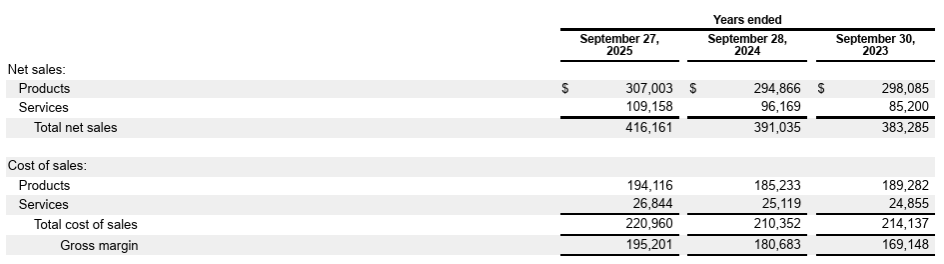
\includegraphics[height=0.5\textheight, keepaspectratio]{pic/fig1.png}
    \end{figure}
\end{frame}

\begin{frame}{Motivation: Financial Numbers and Narrative Text}
    \begin{figure}
        \centering
        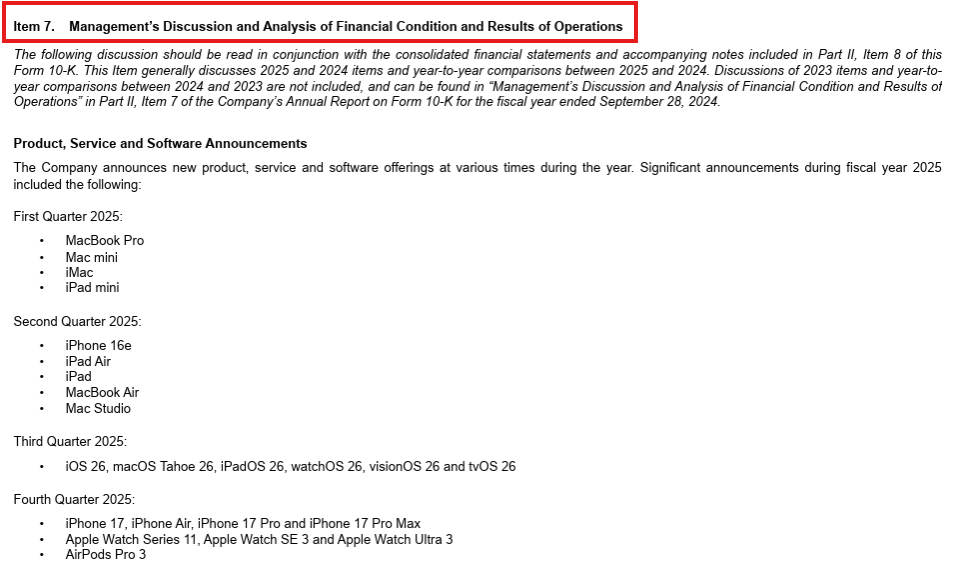
\includegraphics[height=0.8\textheight, keepaspectratio]{pic/fig2.png}  
    \end{figure}
\end{frame}

\begin{frame}{Motivation: Financial Numbers and Narrative Text}
    \begin{figure}
        \centering
        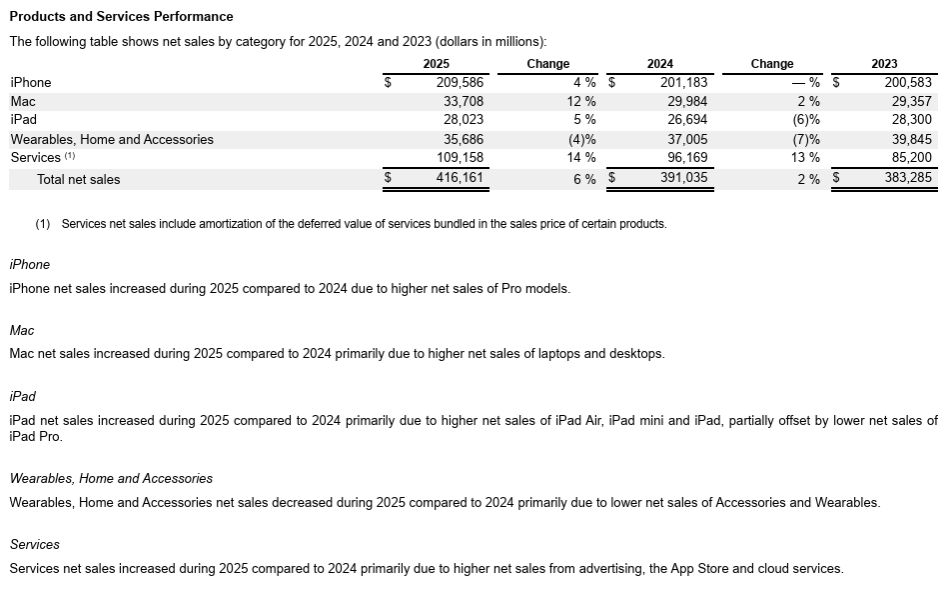
\includegraphics[height=0.8\textheight, keepaspectratio]{pic/fig3.png}  
    \end{figure}
\end{frame}

\begin{frame}{Research Gap}
    \begin{columns}
        % Left Column: Concise Text
        \begin{column}{0.45\textwidth}
            \begin{itemize}
                \item \textbf{Prior Studies:} Textual disclosures (e.g., MD\&A) show moderate direct predictive power.
                \item \textbf{Shallow Interactions:} Previous models combine numbers and text using unidimensional features (e.g., readability, sentiment) and simple linear frameworks.
                \item \textbf{Methodological Gap:} Standard methods miss the \textbf{non-linear interactions} between high-dimensional narrative semantics and reported numbers.
            \end{itemize}
        \end{column}
        
        % Right Column: TikZ Diagram
        \begin{column}{0.55\textwidth}
            \begin{figure}
                \centering
                \resizebox{\textwidth}{!}{
                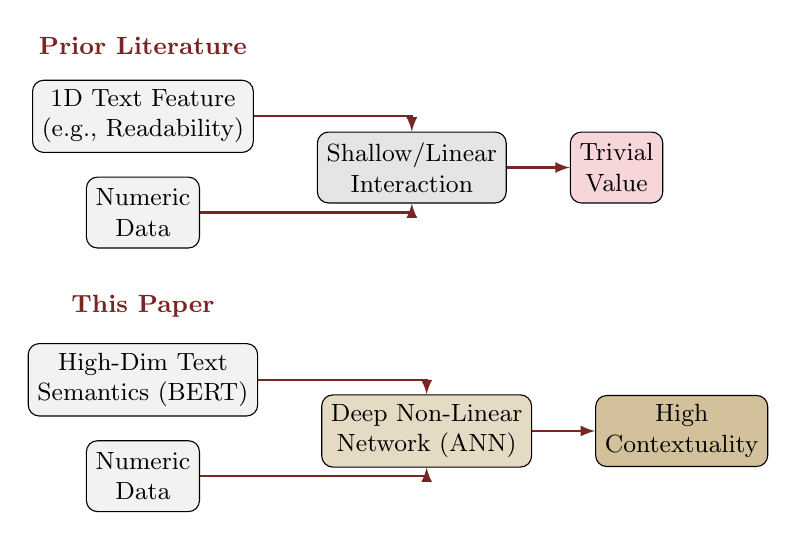
\begin{tikzpicture}[
                    node distance=1.5cm and 0.8cm,
                    box/.style={draw, rounded corners, fill=gray!10, align=center, minimum height=0.9cm, font=\small},
                    arrow/.style={-latex, thick, draw=hkustblue}
                ]
                
                % --- Prior Literature ---
                \node[box] (prior_text) {1D Text Feature \\ (e.g., Readability)};
                \node[box, below=0.3cm of prior_text] (prior_num) {Numeric \\ Data};
                \node[box, fill=gray!20, right=0.8cm of prior_text, yshift=-0.65cm] (linear) {Shallow/Linear \\ Interaction};
                \node[box, fill=hkustred!20, right=0.8cm of linear] (result1) {Trivial \\ Value};

                \draw[arrow] (prior_text) -| (linear);
                \draw[arrow] (prior_num) -| (linear);
                \draw[arrow] (linear) -- (result1);

                \node[above=0.2cm of prior_text, font=\bfseries\small, text=hkustblue] {Prior Literature};

                % --- This Paper ---
                \node[box, below=1.2cm of prior_num] (new_text) {High-Dim Text \\ Semantics (BERT)};
                \node[box, below=0.3cm of new_text] (new_num) {Numeric \\ Data};
                \node[box, fill=hkustyellow!30, right=0.8cm of new_text, yshift=-0.65cm] (deep) {Deep Non-Linear \\ Network (ANN)};
                \node[box, fill=hkustyellow!50, right=0.8cm of deep] (result2) {High \\ Contextuality};

                \draw[arrow] (new_text) -| (deep);
                \draw[arrow] (new_num) -| (deep);
                \draw[arrow] (deep) -- (result2);

                \node[above=0.2cm of new_text, font=\bfseries\small, text=hkustblue] {This Paper};
                
                \end{tikzpicture}
                }
            \end{figure}
        \end{column}
    \end{columns}
\end{frame}

\begin{frame}{Research Question}
    \vspace{0.5cm}
    \begin{center}
        \Large \textit{``To what extent does the \textbf{narrative context} surrounding the numbers in financial statements \textbf{alter the informativeness} of these numbers? (contextualize them?)''}
    \end{center}
    \vspace{0.5cm}
    \begin{itemize}
        \item How economically important are the complementarities between numeric and narrative disclosures in \textbf{shaping investor beliefs}?
        \item \textbf{Under what specific economic circumstances} does narrative context matter the most for interpreting financial data?
    \end{itemize}
\end{frame}

\begin{frame}{Theory and Hypotheses}
    \begin{itemize}
        \item \textbf{Contextualization:} Narrative disclosures contain useful informon and provide a rich context aiming to help investors to understand the reported amounts \citep{bryan1997incremental,li2010information,mayew2015md}. 
        \item \textbf{Interactions:} The qualitative information which may seem immaterial on their own, when \textbf{interacting with financial numbers} in complex ways can be valuable for \textbf{predicting future outcomes}.
    \end{itemize}
\end{frame}

% Research Design --- --- --- --- --- --- --- --- --- --- --- --- 
\section{Research Design}

\begin{frame}{Encoding Narrative Information (BERT)}
    \begin{itemize}
        \item \textbf{Text Extraction:} Extract \textbf{MD\&A sentences} with earnings keywords, plus \textcolor{hkustred}{\textbf{one adjacent sentence}} on each side for context.
        \item \textbf{Encoding Process:} Divide text into passages of up to 512 tokens and process via a pre-trained \textcolor{hkustred}{\textbf{BERT-base uncased model}}.
        \item \textbf{Why BERT?:} Unlike bag-of-words, BERT uses \textcolor{hkustred}{\textbf{self-attention}} to dynamically learn semantic meaning, capturing the \textbf{high-dimensional, complex narratives} in financial disclosures.
    \end{itemize}
\end{frame}

\begin{frame}{Modeling Contextualized Interpretation (ANN)}
    \begin{itemize}
        \item \textbf{The Mechanism:} Deploy an \textbf{Artificial Neural Network (ANN)} to capture the \textcolor{hkustred}{\textbf{deep, highly nonlinear interactions}} between textual features and accounting numbers.
        \item \textbf{Network Architectures:}
        \begin{itemize}
            \item \textbf{Fully Connected:} Contextual neurons directly \textcolor{hkustred}{\textbf{influence the activation}} of numeric neurons, allowing the narrative to effectively \textit{contextualize} the numbers.
            \item \textbf{Partially Connected:} Restricts cross-layer interactions, isolating the standalone (direct) value of the text as a baseline.
        \end{itemize}
    \end{itemize}
\end{frame}

\begin{frame}{Neural Network Architectures}
    \begin{columns}[T] % The [T] aligns the columns at the top
        
        % Left Column: Figure 4
        \begin{column}{0.5\textwidth}
            \begin{figure}
                \centering
                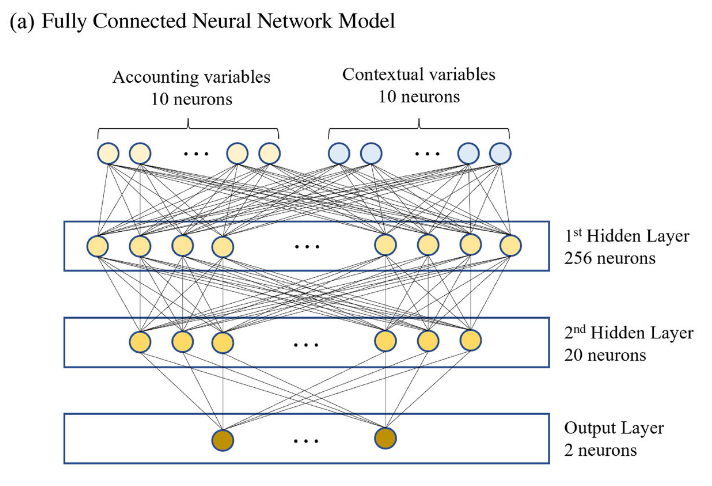
\includegraphics[width=1\textwidth, keepaspectratio]{pic/fig4.png}
                \vspace{0.2cm}
            \end{figure}
        \end{column}
        
        % Right Column: Figure 5
        \begin{column}{0.5\textwidth}
            \begin{figure}
                \centering
                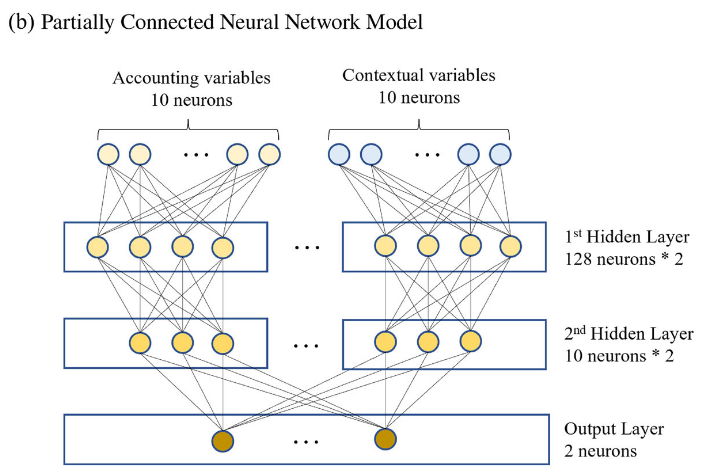
\includegraphics[width=1\textwidth, keepaspectratio]{pic/fig5.png}
                \vspace{0.2cm}
            \end{figure}
        \end{column}
    \end{columns}
    \small In the fully connected model, each neuron stemming from textual input participates in the activation of numeric neurons. This allows two types of input to \textcolor{hkustred}{\textbf{interact in complex ways}}.
\end{frame}

\begin{frame}{Data Collection and Processing}
    \begin{itemize}
        \item \textbf{Sample Construction:} Analyzed machine-readable SEC \textbf{MD\&A filings from 1995 to 2021}, merging textual data with Compustat (financials) and CRSP (returns).
        \item \textbf{Narrative Extraction:} Identified sentences containing earnings-related keywords and extracted \textbf{one adjacent sentence on each side} to capture the context.
        \item \textbf{BERT Encoding:} Processed the extracted text in 512-token passages through a \textbf{BERT-base uncased model}. Averaged the output CLS token vectors to create a \textbf{768-dimensional context vector} for each MD\&A.
        \item \textbf{Final Sample:} Yielded 87,201 firm-year observations for earnings/cash flow tests and 62,287 observations for stock return predictions.
    \end{itemize}
\end{frame}

\begin{frame}{Model Design (ANN Architecture)}
    \begin{itemize}
        \item \textbf{Target Variable ($T_{t+1}$):} Predicts directional changes (increase/decrease) in future performance (earnings, cash flows, or stock returns). 
        \item \textbf{Model Inputs:} 
        \begin{itemize}
            \item \textcolor{hkustred}{\textbf{Accounting Vector ($A_t$):}} 10D vector of current and lagged earnings and OCF. 
            \item \textcolor{hkustred}{\textbf{Context Vector ($C_t$):}} 10D CLS vector compressed from the 768D BERT output. 
        \end{itemize}
        \item \textbf{Function:} $E_{t}[T_{t+1}|A_{t},C_{t}]=\Lambda_{t}(A_{t},C_{t})$, where deep nonlinear interactions contextualize the numbers.
        \item \textbf{Network Architectures:} 
        \begin{itemize}
            \item \textcolor{hkustred}{\textbf{Fully Connected:}} All neurons interact (256 $\rightarrow$ 20 $\rightarrow$ 2). Text directly influences the interpretation of numbers. 
            \item \textcolor{hkustred}{\textbf{Partially Connected:}} Restricts interactions (e.g., split 128/128 in Hidden Layer 1). Isolates the standalone value of text. 
        \end{itemize}
        \item \textbf{Contextuality Measure:} Evaluated as the \textcolor{hkustred}{\textbf{difference in accuracy}} between the fully connected and partially connected models. 
    \end{itemize}
\end{frame}

% Results --- --- --- --- --- --- --- --- --- --- --- 
\section{Results}

\begin{frame}{Predicting Future Fundamentals: Earnings \& Cash Flows}
    \begin{figure}
        \centering
        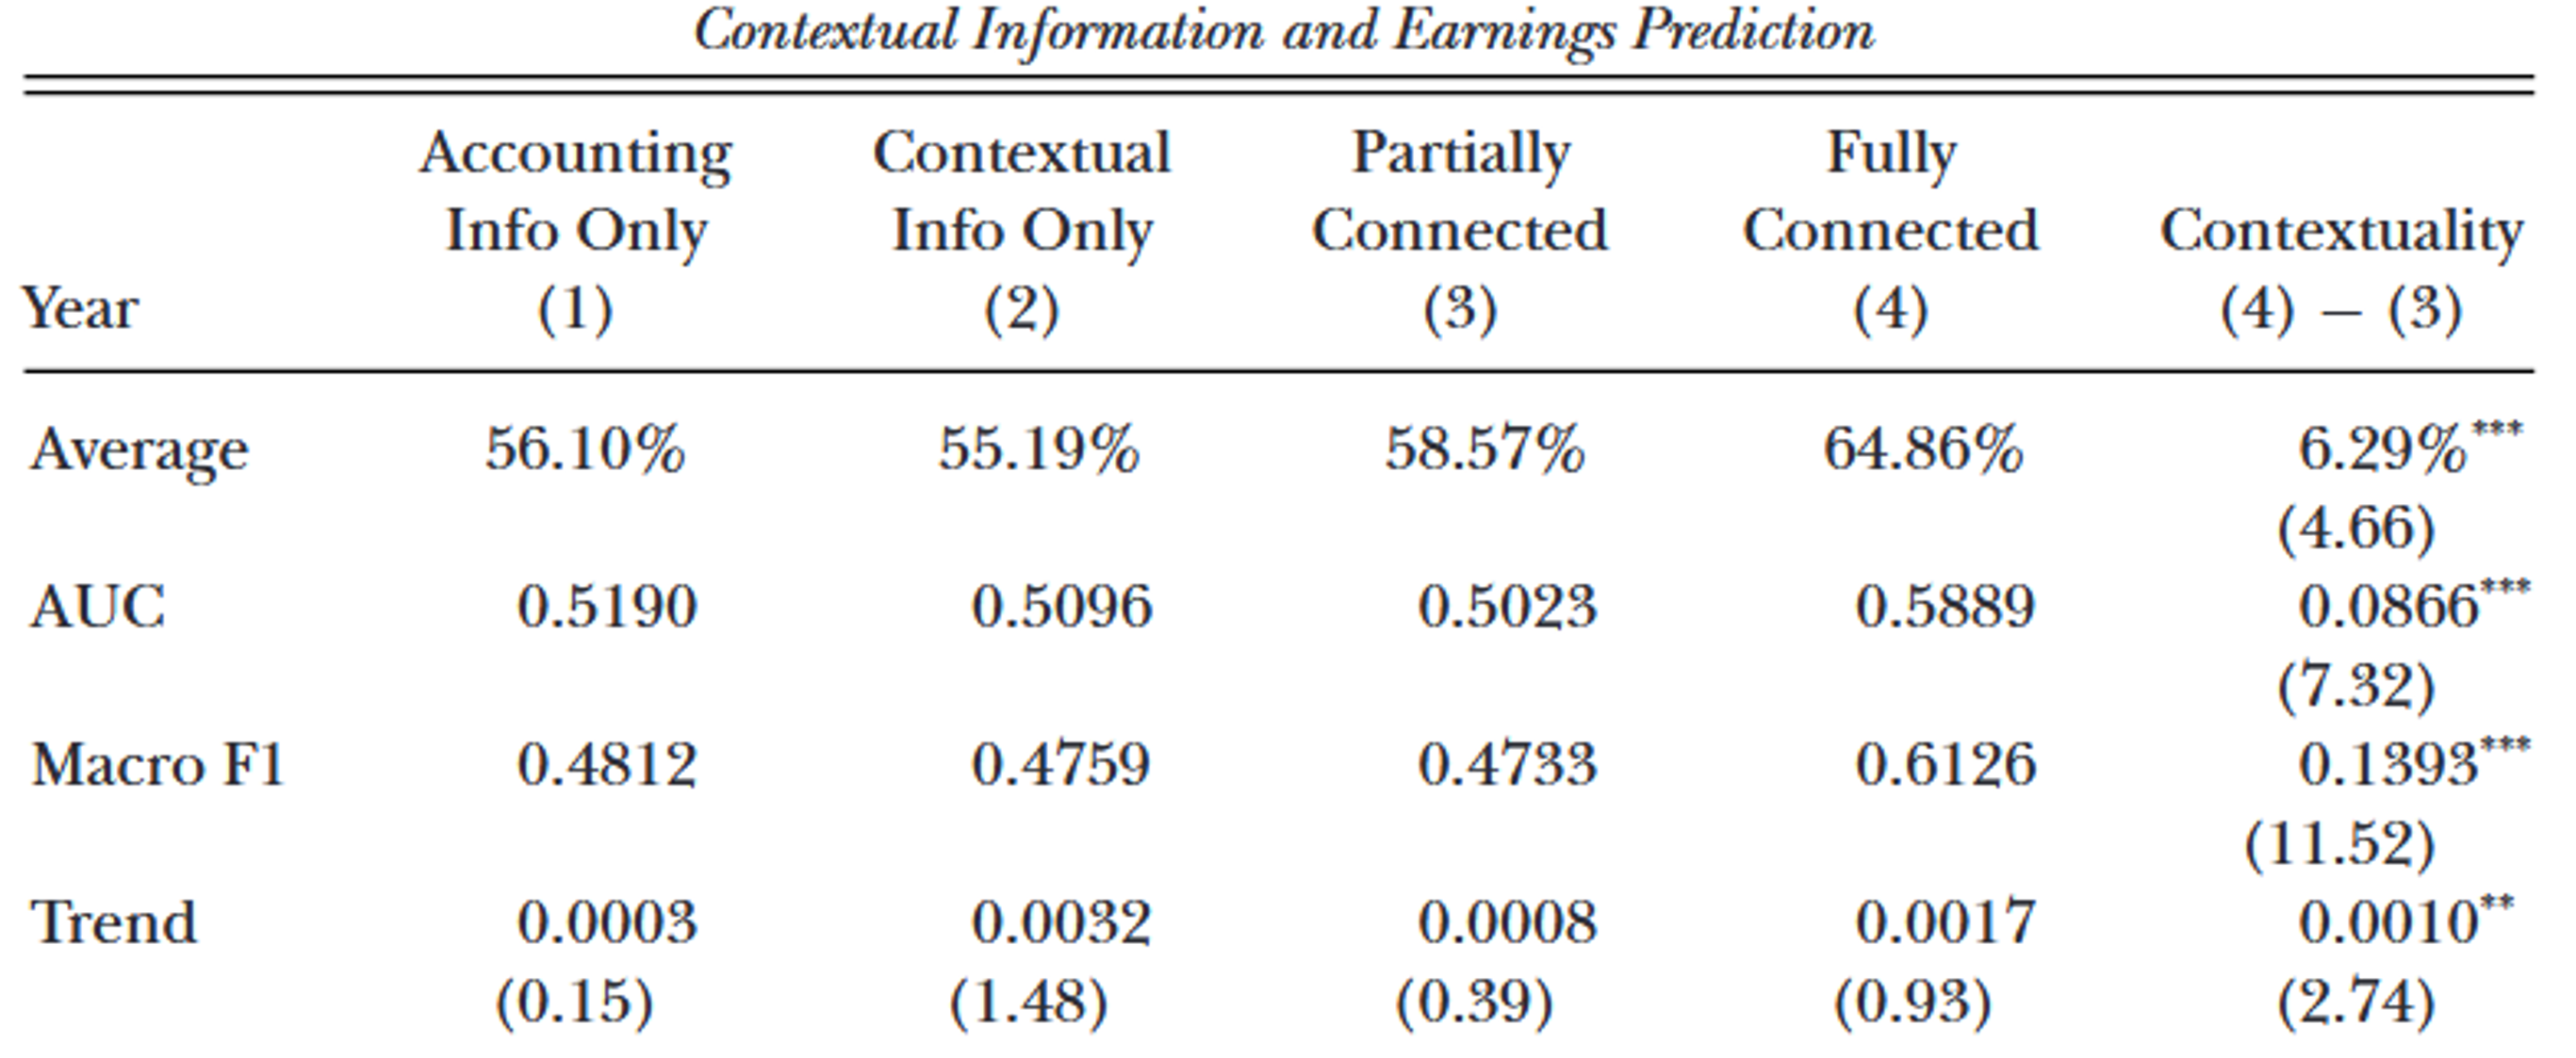
\includegraphics[width=0.48\textwidth, keepaspectratio]{pic/tab3.png}
        \hfill
        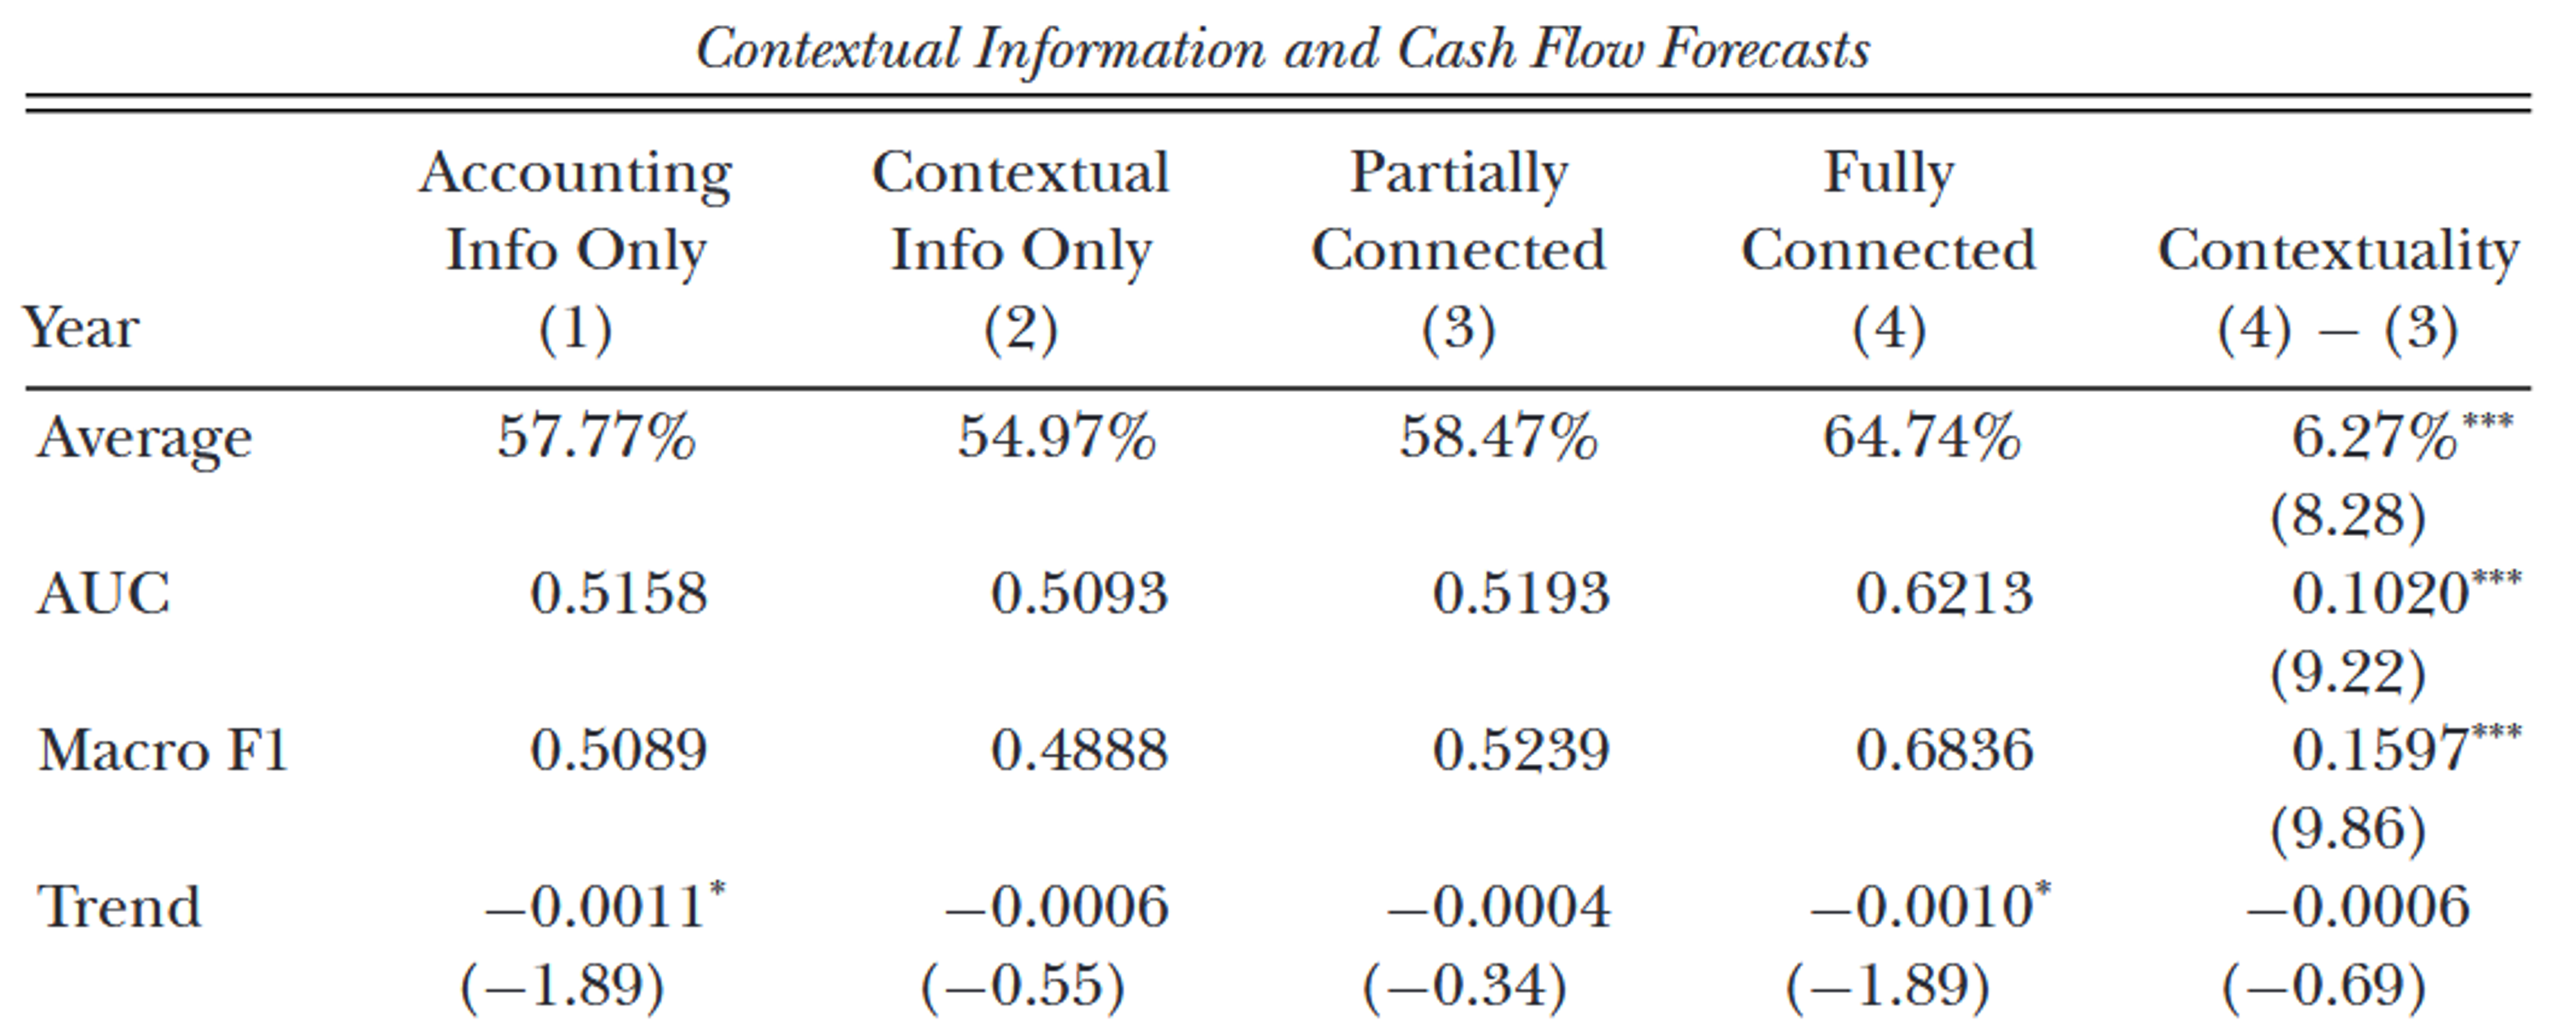
\includegraphics[width=0.5\textwidth, keepaspectratio]{pic/tab4.png}
    \end{figure}
    
    \vspace{-0.2cm} % Adjust this value if you need more or less space between the image and text
    
    \begin{itemize}
        \item \textbf{Directional Prediction:} The fully connected model achieves an accuracy of \textbf{64.86\%} \& \textbf{64.74\%} in earnings and OCF forecast.
        \item \textbf{Performance Metrics:} Area Under the ROC Curve (AUC) and Macro F1-scores confirm the model minimizes both Type I and Type II errors.
        \item \textbf{Time Trend:} Evaluated via the regression $Dep\_Var_{t}=\lambda_{0}+\lambda_{1}Time_{t}+\epsilon_{t}$. 
        The contextuality of earnings exhibits a \textbf{positive and statistically significant growth trend} ($\lambda_1 > 0$), indicating narrative context is increasingly important over time.
    \end{itemize}
\end{frame}

\begin{frame}{Stock Return: Does Market Recognize the Context?}
\begin{figure}
        \centering
        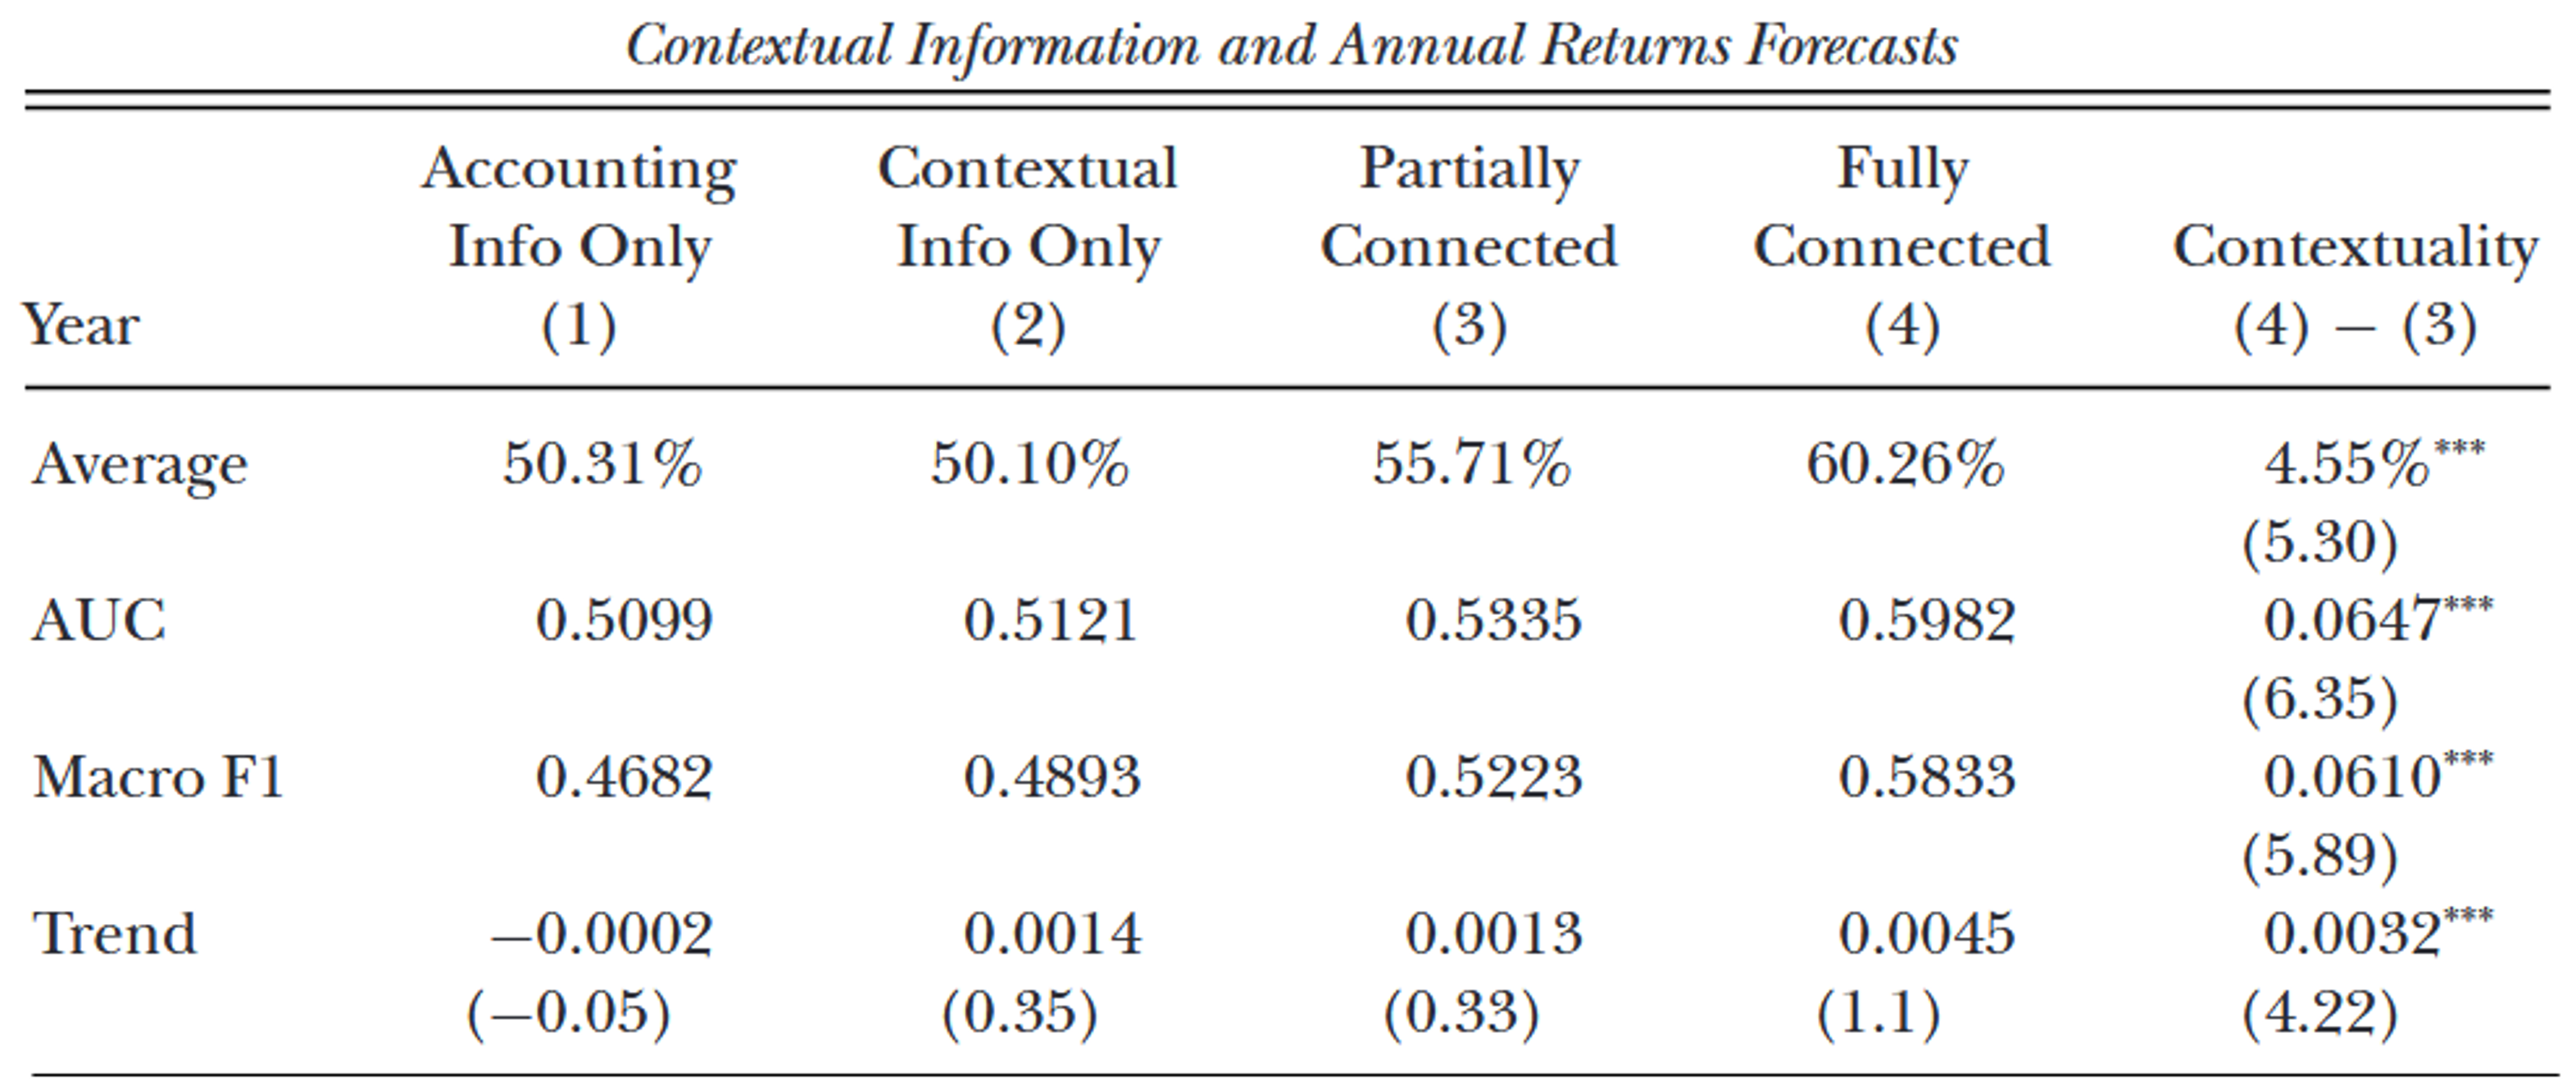
\includegraphics[width=0.48\textwidth, keepaspectratio]{pic/tab5.png}
        \hfill
        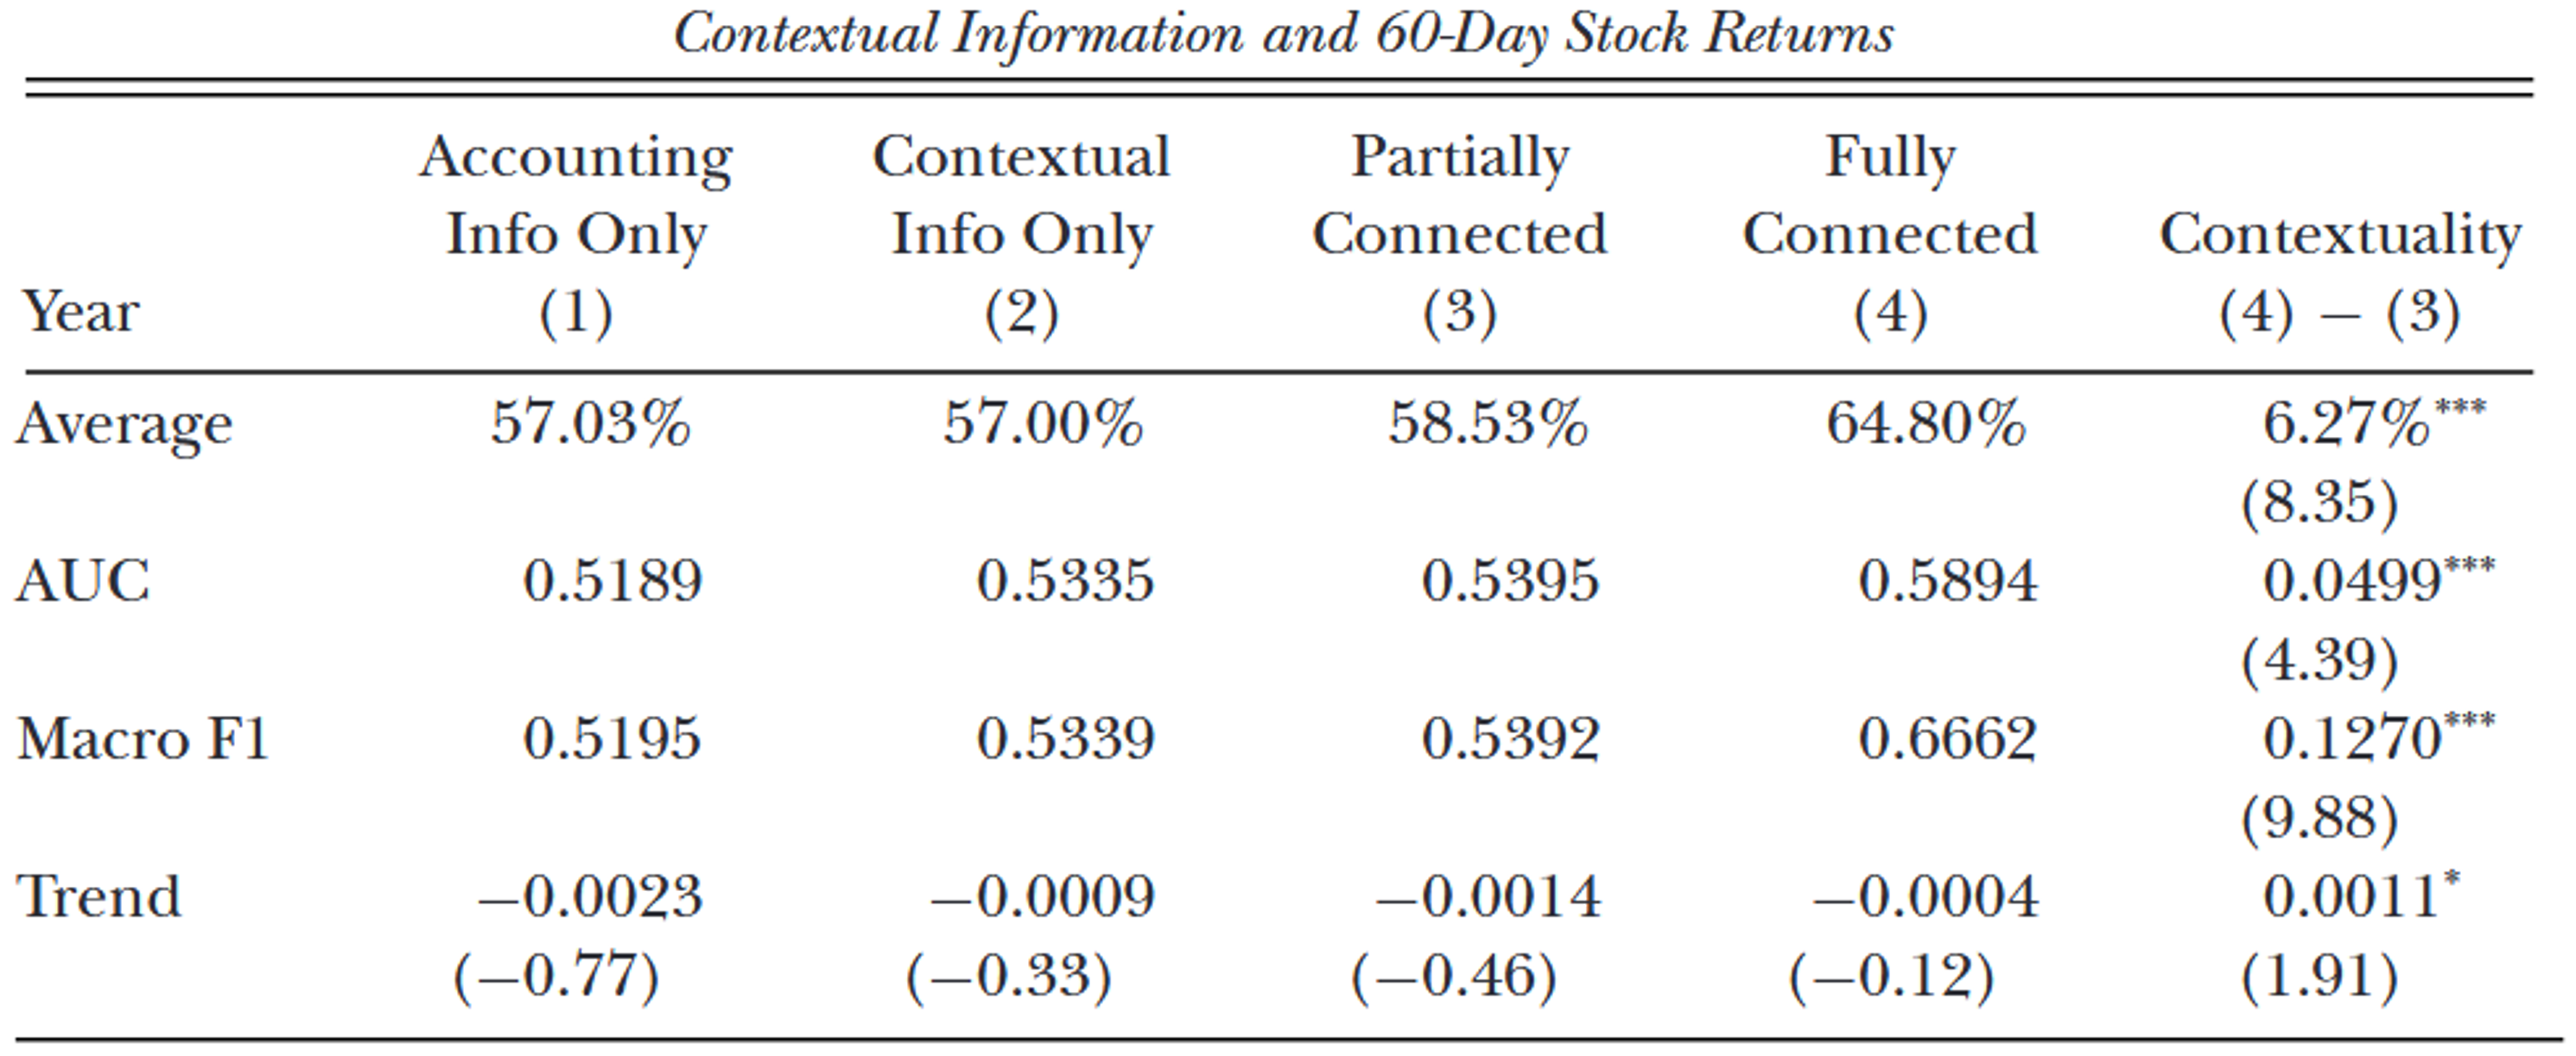
\includegraphics[width=0.5\textwidth, keepaspectratio]{pic/tab6.png}
    \end{figure}
    
    \vspace{-0.2cm} 
    \begin{itemize}
        \item \textbf{Annual Returns (Longer Window):} Incorporating context interactions improves long-window return predictions by over 4.5 percentage points.
        \item \textbf{60-Day Returns (Post-Filing):} Excludes the initial earnings surprise to focus on the MD\&A details. The fully connected model yields an \textbf{11\% increase} in accuracy.
        \item \textbf{Takeaway:} The stock market actively prices the nonlinear interactions between reported financials and narrative text.
    \end{itemize}
\end{frame}

\begin{frame}{When Does Context Matter Most?}
\begin{figure}
        \centering
        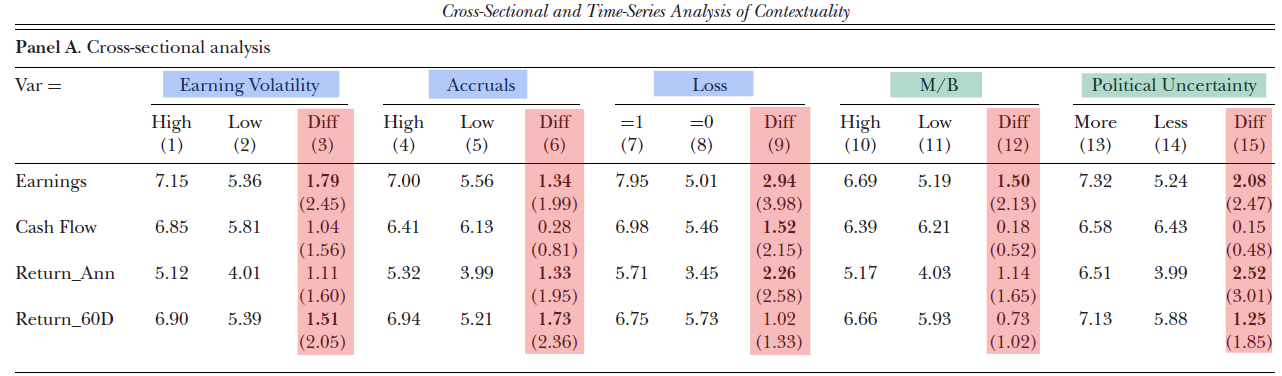
\includegraphics[width=0.9\textwidth, keepaspectratio]{pic/tab7.1.png}
    \end{figure}
    \vspace{-0.2cm}
    \begin{itemize}
        \item \textbf{Firm-Level Uncertainty (Cross-Sectional):} Contextual information becomes significantly more valuable when the numeric data is 1) less likely to be forward-looking or 2) is harder to evaluate. Proxies:
        \begin{itemize}
            \item 1): High earnings volatility \citep{dichev2009earnings}, extreme accruals (top/bottom 20\%) \citep{sloan1996stock}, reported operating losses \citep{hayn1995information}.
            \item 2): M/B ratio \citep{beaver2005conditional}, political risk \citep{hassan2019firm}.
        \end{itemize}
    \end{itemize}
\end{frame}

\begin{frame}{When Does Context Matter Most?}
\begin{figure}
        \centering
        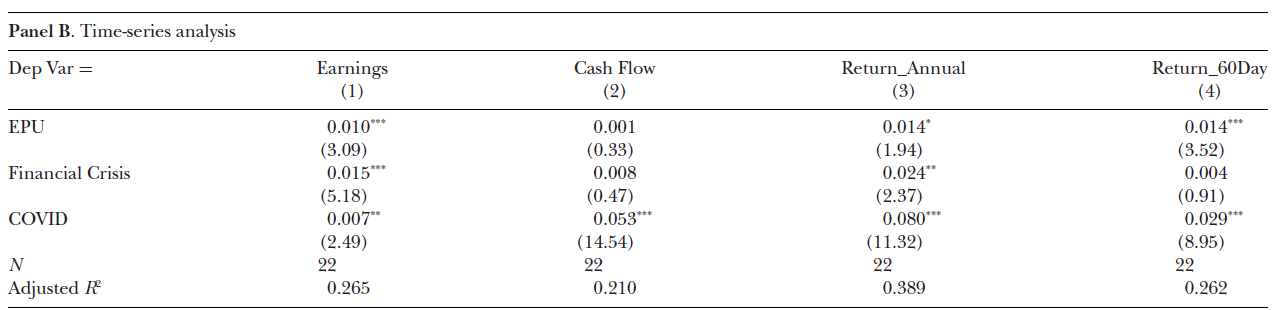
\includegraphics[width=1.0\textwidth, keepaspectratio]{pic/tab7.2.png}
    \end{figure}
    \begin{itemize}
        \item \textbf{Macro-Level Uncertainty (Time-Series):} Contextuality spikes during periods when it is difficult to map accounting numbers to valuations. Regress annual average contextuality on three variables:
        \begin{itemize}
            \item The 2008 Global Financial Crisis.
            \item The COVID-19 Pandemic (2020).
            \item Periods of high Economic Policy Uncertainty (EPU).
        \end{itemize}
    \end{itemize}
\end{frame}

\begin{frame}{Human Validation: Security Analysts}
\begin{figure}
        \centering
        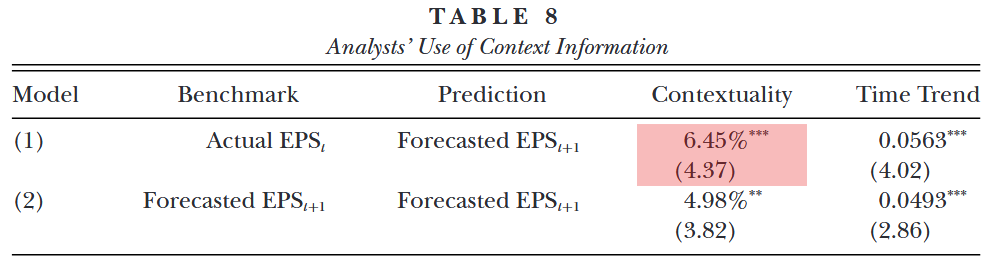
\includegraphics[width=1.0\textwidth, keepaspectratio]{pic/tab8.png}
    \end{figure}
    \begin{itemize}
        \item \textbf{Hypothesis:} If contextualization is real, human decision-makers (analysts) should also rely on these interactions when revising their forecasts.
        \item \textbf{Findings:} The fully connected ANN model explains analysts' forecast revisions significantly better than models lacking textual interaction.
        \item It yields a \textbf{6.45 percentage point increase} in explanatory power over forecast revisions (using actual EPS benchmark).
    \end{itemize}
\end{frame}

\begin{frame}{Application: Contextualized Earnings Persistence}
    \begin{itemize}
        \item \textbf{The Challenge:} Standard earnings persistence measures rely on rigid rolling windows (context-free) and fail to capture dynamic, firm-year specific changes.
        \item \textbf{The Approach:} The authors model the persistence parameter as a \textcolor{hkustred}{\textbf{nonparametric function of high-dimensional textual vectors}} using deep learning.
        \item \textbf{Rich Heterogeneity:} This context-based measure uncovers substantial firm-year variation in earnings quality that standard firm characteristics (e.g., size, M/B) cannot explain.
        \item \textbf{Predictability:} Context-based persistence significantly outperforms traditional models in predicting \textbf{out-of-sample} earnings dynamics.
        \item \textbf{Economic Magnitude:} Incorporating the narrative context reduces the \textcolor{hkustred}{\textbf{Mean Absolute Error (MAE) by over 50\%}} (from 5.65 down to 2.21) compared to context-free estimates.
    \end{itemize}
\end{frame}

% Discussion --- --- --- --- --- --- --- --- --- --- --- --- 
% Discussion --- --- --- --- --- --- --- --- --- --- --- --- 
\section{Discussion}

\begin{frame}{Contributions}
    \begin{itemize}
        \item \textbf{Methodological Innovation:} Introduces a novel deep learning approach \textcolor{hkustred}{\textbf{(BERT + ANN)}} to quantify the \textit{contextuality} of textual disclosures, moving beyond unidimensional features like readability or sentiment.
        \item \textbf{Economic Magnitude:} Quantifies the \textcolor{hkustred}{\textbf{(collective value of numeric-narrative interactions)}}, proving they are economically large.
        \item \textbf{Textual Analysis of Corporate Communications:} Answers the call in literature to apply deep learning to capture unknown, high-dimensional features and \textcolor{hkustred}{\textbf{(complex nonlinearities)}} in accounting data.
        \item \textbf{New Accounting Metric:} Develops a dynamic, firm-year specific measure of \textcolor{hkustred}{\textbf{context-based earnings persistence}} that outperforms traditional rolling-window OLS estimates.
    \end{itemize}
\end{frame}

\begin{frame}{Strengths \& Weaknesses}
    \begin{columns}[T]
        \begin{column}{0.48\textwidth}
            \textbf{\textcolor{hkustred}{Strengths}}
            \begin{itemize}
                \item \textbf{ANN Architecture:} Mimics human cognitive processing by allowing deep interactions across neural layers.
                \item \textbf{Rich Results:} Evaluates multiple fundamental (earnings, OCF) and market (returns) targets over a long sample period (1995-2021).
                \item \textbf{Practical Application:} Validates the methodology by solving a real-world accounting challenge (measuring firm-year earnings persistence).
            \end{itemize}
        \end{column}
        
        \begin{column}{0.48\textwidth}
            \textbf{\textcolor{teal}{Weaknesses \& Limitations}}
            \begin{itemize}
                \item \textbf{The "Black Box" Problem:} While highly predictive, ANNs offer limited explaination regarding \textit{which} specific words or phrases drive the results (like RFs).
                \item \textbf{Scope Limitation:} Focuses exclusively on MD\&A sections, potentially missing context from other filing sections or earnings call Q\&A transcripts.
            \end{itemize}
        \end{column}
    \end{columns}
\end{frame}

\begin{frame}{Future Research Directions}
    \begin{itemize}
        \item \textbf{Vocal Cues \& Narrative Context:} Extending the methodology to examine how managerial vocal cues (affective states) provide context to oral narratives during earnings conference calls (Katrina's presentation on vocal delivery quality ).
        \item \textbf{Detecting Deception:} Exploring interactions between verbal communications and nonverbal cues (e.g., gestures, facial expressions, body language) to detect fraudulent reporting and deceptive practices (Xi Zhen's presentation on CEO facial expressions).
        \item \textbf{Accounting Quality \& Manipulation:} Applying the context-based persistence framework to better evaluate overall earnings quality and detect earnings manipulation.
        \item \textbf{Cross-Regime Comparisons:} Using this approach to compare the usefulness of context across different regulatory disclosure regimes.
    \end{itemize}
\end{frame}

% References
\begin{frame}[allowframebreaks]{References}
    \bibliographystyle{plainnat} 
    \bibliography{reference} 
\end{frame}

%------------------------------------------------

\begin{frame}
    \Huge{\centerline{\textbf{Thanks}}}
\end{frame}

%----------------------------------------------------------------------------------------

\end{document}